\documentclass[xcolor=table]{beamer}

\usepackage[polish]{babel}
\usepackage[utf8]{inputenc}
\usepackage[T1]{fontenc}
\usepackage{listings}
\usepackage{lmodern}
\usepackage{textcomp}


\usetheme[language=polish]%
  {Goddard}

\newcommand{\filepath}{\texttt}
\newcommand{\command}{\texttt}
\newcommand{\email}[1]{\href{mailto:#1}{\texttt{#1}}}
\newcommand{\latexcode}{\texttt}
\newcommand{\parameter}[1]{\textlangle #1\textrangle}


\lstset{basicstyle=\ttfamily,keywordstyle=\color{goddardblue}\bfseries,commentstyle=\color{goddardblue!75}\itshape,columns=flexible}

\rowcolors{1}{goddardblue!50}{goddardblue!30}


\title{Szyfrowanie SMS’ów}
\subtitle{technologia oraz przegląd algorytmów}
\author{Bartłomiej Bułat\\
Tomasz Czarnik\\
Krzysztof Śmiłek\\}


\begin{document}

%==============================
\begin{frame}
  \titlepage
\end{frame}


%==============================
\begin{frame}
  \frametitle{Plan}
  \tableofcontents
\end{frame}


%=============================================================
\section{Wstęp}

\begin{frame}
  \frametitle{Wstęp}
 Krótkie wiadomości tekstowe potocznie zwane SMS (Short Message Service) na dobre zadomowiły się w większej części świata i stanowią dzisiaj jeden z popularniejszych kanałów komunikacji. 
% można tu umieścić komiks z XKCD lub dane z niego w porównaniu do całego Internetu 
% bathez: który komiks?
\end{frame}

\subsection{Zastosowania}
%==============================
\begin{frame}
  \frametitle{Zastosowania}

Stosowane są m. in. do:
\begin{itemize}
\item Wysyłania krótkich wiadomości i ``"czatów''
\item Aktywowania usług u operatorów komórkowych
\item Powiadomień od operatorów, banków i innych instytucji
\item Wysyłania bezpiecznych tokenów - haseł
\item Reklam i konkursów SMS
\item Sterowania urządzeniami 
%kamerki szpiegowskie hehe
\end{itemize}
   
\end{frame}

%=============================================================
\section{Technologia}

%=============================================================
\subsection{Krótka historia GSM}
\begin{frame}[allowframebreaks]
  \frametitle{Krótka historia GSM}

  Pierwsza specyfikacja (GSM 900 Phase 1)
  \begin{itemize}
    \item \textbf{1982 r.} - powstanie instytutu Groupe Spécial Mobile, 2 lata
      później - projekt specyfikacji
    \item \textbf{1987 r.} - derektywa unijna o rezerwacji czestotliwości przez
      państwa członkowskie, rok później - specyfikacja GSM 900 Phase 1
    \item \textbf{1989 r.} - powstanie \emph{Europejskiego Instytutu Norm
      Telekomunikacyjnych (ETSI)}, przejecie prac nad standardem, rok później -
      domknięcie standardu i rozpoczecie budowy infrastruktury
  \end{itemize}

  \framebreak

  Specyfikacja GSM Phase 2
  \begin{itemize}
    \item \textbf{1990 r.} - opracowanie specyfikacji GSM 1800 (DCS).
      Uwzględnienie przesyłania SMS-ów i danych.
    \item \textbf{1991 r.} - pierwsze połączenie telefoniczne w standardzie GSM
    \item \textbf{1993 r.} - uruchomienie DCS w Wielkiej Brytani oraz pierwsze
      uruchomienie GSM poza Europą
    \item \textbf{1995 r.} - zakończenie prac nad standardem GSM Phase 2
  \end{itemize}
\end{frame}

%=============================================================
\subsection{Wiadomości SMS}

\begin{frame}
  \frametitle{Powstanie SMS}

  \begin{itemize}
    \item \textbf{1982 r.} - grupa GSM proponuje system wymiany wiadomości
      tekstowych miedzy stacjami nadawczymi lub za pomocą protokołu Message
      Handling System (wtedy bardzo popularnego)
    \item \textbf{1984 r.} - opracowanie koncepcji SMS-a jako widomości o
      długości 160 znaków wykorzystujacy do przesyłania kanał informacyjny
      (nieużywany przez większość czasu komunikacji urzadzeń) - przez Deutsche
      Telekom oraz France Télécom.
    \item \textbf{grudzień 1992 r.} - pierwszy SMS o treści ``Merry
      Christmas''
  \end{itemize}
\end{frame}

\begin{frame}
  \frametitle{Centra SMS}

  W pierwszych implementacjach SMS wiadomości były dostarczana kanałem
  informacyjnym bezpośrednio do odbiorcy. W póxniejszych implementacjach stacji
  GSM dodano obsługę \emph{centr SMS (SMSC)}. Każdy wysłany SMS trafia do
  centrum które wysyła widomość do odbiorcy gdy ten znajduje się zasięgu sieci,
  jesli nie wiadomość oczekuje do momentu zalogowania się odbiorcy. Jesli minie
  czas ważnosci wiadomości SMS nie jest dostarczany.
\end{frame}

\begin{frame}
  \frametitle{Popularność SMS}

  \begin{center}
    \begin{figure}
      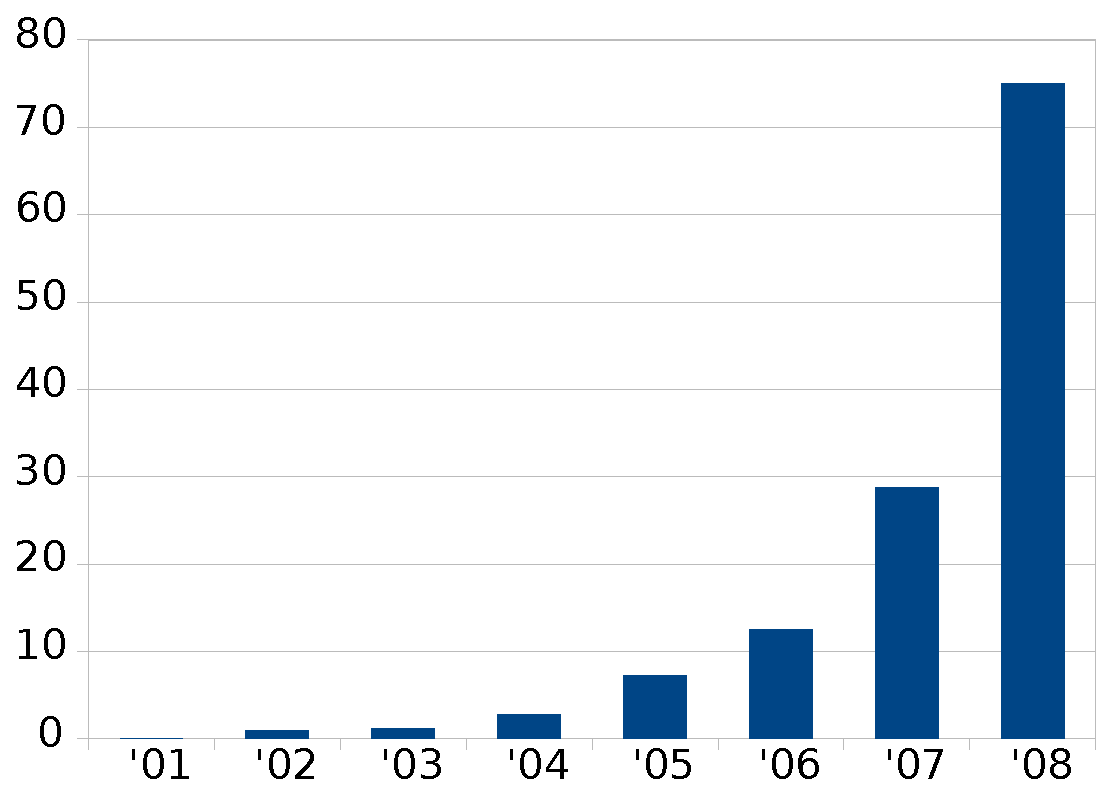
\includegraphics[width=0.7\textwidth]{sms_sent_monthly}
      \caption{Liczba wysłanych SMS-ów miesięcznie w USA w latach 2001 - 2008
      (w miliardach)}
    \end{figure}
  \end{center}
\end{frame}


%==============================
\subsection{Ograniczenia}
\begin{frame}[allowframebreaks]
  \frametitle{Liczba znaków}

  Poczatkowo SMS pozwalał na wysłanie 128 znaków (128 oktetów - 1024 bity).
  Mastepnie udało się rozszerzyć protokuł do 140 oktetów (1120 bitów).
  Zmieniając kodowanie znaków na tzw. alfabet GSM, który używa 7 bitów na znak
  udaje się wysłać 160 znaków w jednej wiadomości.

  \textbf{Liczba 160 znaków} ma podłoże w badaniach przeprowadzonych na
  widomościach przesyłanych pocztówkami i przez dalekopisy. Analiza długości
  pozwoliła stwirdzić, że do tego typu komunikacji potrzeba ok. 150 znaków.
  Liczba natomiast 160 wynika ze specyfiki technologii.

  \framebreak

  \textbf{Alfabet GSM} - okrojona tablica ASCII do 127 pierwszych znaków, gdzie
  większość znaków sterujących została zastąpiona znakami z drugiej częsci
  tablicy ASCII.

\end{frame}
%=============================================================
\begin{frame}
  \frametitle{Problem znaków spoza alfabetu GSM}

  Współczesne urządzenia domyslnie wysyłają SMS w alfabecie GSM, jesli jednak
  użyjemy znaku który znajduje się poza tym alfabetem (np. znaku z ogonkiem)
  widomośc zostanie wyslana w kodowaniu LATIN-1 (dla polskiego alfabetu), które
  jest kodowaniem 8-bitowym, co zmniejsza pojemnośc SMS-a do 140 znaków.

  Jeśli chcemu użyć znaków z języków takich jak japoński, chiński, arabski czy
  cyrylicy nalezy użyć kodowania 16-bitowego UCS-2 co jednak redukuje pojemność
  SMS do 60 znaków.

  Niektóre nowoczesne telefony domyślnie przłaczają się do kodowania UCS-2
  jeśli użyjemy znaku spoza alfabetu GSM.
\end{frame}

%==============================
\begin{frame}
  \frametitle{Wielostronnicowe SMS}

lorem ipsum i takie tam

\end{frame}

%=============================================================
\subsection{Zagrożenia}
\begin{frame}
  \frametitle{Zagrożenia}

\begin{itemize}
\item Sposoby podsłuchu 
%np. zdjęcie urządzenia podsłuchowego
\item Podszywanie się pod numery
\end{itemize}

\end{frame}

%=============================================================
\section{SMS od podszewki}
%=============================================================

\subsection{Modemy}
\begin{frame}
  \frametitle{Telefony i modemy 3G}

lorem ipsum i takie tam

\end{frame}
%=============================================================

\begin{frame}
  \frametitle{Bluetooth DUN}

lorem ipsum i takie tam

\end{frame}
%=============================================================
\subsection{Komendy AT}
\begin{frame}
  \frametitle{Komendy AT}

lorem ipsum i takie tam

\end{frame}
%=============================================================

\begin{frame}
  \frametitle{Zestawy komend}

lorem ipsum i takie tam

\end{frame}
%=============================================================
\begin{frame}
  \frametitle{Komendy służące do obsługi SMS}

lorem ipsum i takie tam

\end{frame}
%=============================================================
\begin{frame}
  \frametitle{Kodowanie znaków}

lorem ipsum i takie tam

\end{frame}

%=============================================================
\section{Szyfrowanie}
%=============================================================

\subsection{Kryteria wyboru}
\begin{frame}
  \frametitle{Kryteria wyboru}

 wymagania, szyfrowanie symetryczne/asymetryczne i dlaczego (przede wszystkim kompresja i ograniczona liczba znaków )

\end{frame}

%=============================================================

\subsection{Przegląd algorytmów}


\begin{frame}
  \frametitle{Szyfr T9}

lorem ipsum i takie tam

\end{frame}

\begin{frame}
  \frametitle{Przykład}

lorem ipsum i takie tam

\end{frame}

%=============================================================
\begin{frame}
  \frametitle{Szyfr cezara}

lorem ipsum i takie tam

\end{frame}

\begin{frame}
  \frametitle{Przykład}

lorem ipsum i takie tam

\end{frame}

%=============================================================
\section{Porównianie}
%=============================================================

\begin{frame}
  \frametitle{Porównanie}
    \begin{itemize}
\item Metoda z użyciem T9, nie wymaga oprogramowania, łatwa w złamaniu
\item Szyf cezara, wyjątkowo prosty i nie narzuca dodatkowych danych
\end{itemize}

\end{frame}

%=============================================================
\section{Podsumowanie}

\begin{frame}
  \frametitle{Podsumowanie}
Spośród omawianych przez nas metod każda ma zalety, ale też pewne słabościi.\\[\baselineskip] Przedstawione technologie i sposoby pozwalają łatwo wprowadzić szyfry i zaimplementować je np. w programie komputerowym korzystającym z modemu 3G lub działającym bezpośrednio na urządzeniu (np. pod systemem Android).

\end{frame}

\end{document}
